%%  Round twenty-two.  The review's ninth comment asks for a thirty-five to
%%  forty page article.  Three results of Section~6 are summarised there in a
%%  paragraph each and reported here in full: the crossing that separates the
%%  model family from the encoding, the decision-rule comparison, and the
%%  calibration, unseen-category and rolling-origin diagnostics.

\subsection{The pipeline axis is two axes}
\label{app:axes2full}

\begin{table}[t]
\centering
\small
\resizebox{\ifdim\width>\linewidth\linewidth\else\width\fi}{!}{%%
\begin{tabular}{llrrrrrr}
\toprule
log & target & encoding & family & quality level & rung & split & higher-order \\
\midrule
BPIC14 & duration & 0.091 & 0.066 & 0.065 & 0.492 & 0.014 & 0.271 \\
BPIC14 & handover & 0.125 & 0.049 & 0.109 & 0.430 & 0.009 & 0.276 \\
\bottomrule
\end{tabular}%
}
\caption{The decomposition with the model family and the encoding as separate axes, on the case study's log where all six pipelines run. First-order shares, median over the five instruments, under the equal-level measure, then the total higher-order share. The `learner' axis of Table~\ref{tab:sobol} is the two of them together.}
\label{tab:axes2}
\end{table}


Table~\ref{tab:sobol}'s ``learner'' column is not a learner axis. Its levels
are pipelines: a model family together with an encoding and, in one case, a
calibration. On \nPairsTwoLearners\ of the \nPairs\ pairs only two of them
run, so the index is a statement about a two-level axis whose levels differ in
two things at once.

On the case study's log the budget allows the two to be crossed. Both model
families --- penalised logistic regression and histogram gradient boosting ---
are run against all three encodings: one-hot, frequency, and cross-fitted
target encoding, on both of the log's targets. That is \nPipelines\ complete
factorial pipelines, and the decomposition of Section~\ref{sec:sobol} then
carries a family axis and an encoding axis separately.

Three things follow, and the third is the reason the confound mattered.

\textbf{The encoding is the larger of the two.} It carries \sEncodingPct\ of
the variance in the increment against the family's \sFamilyPct. How the
register is turned into columns matters about twice as much as which model
consumes them, and it is the choice more often left unstated.

\textbf{Their interaction is as large as either main effect.} The
family--encoding two-way component carries \sFamilyEncodingPct, the largest
two-way term in the crossed decomposition. A gradient-boosting model and a
logistic model do not respond to a change of encoding in the same way, which
is precisely what an axis that fuses them cannot express.

\textbf{So the fused index is not the sum of two indices.} It is a statement
about a two-level axis whose levels move two things at once, and
Table~\ref{tab:sobol}'s pipeline column should be read as that and nothing
more. The crossing has not been re-run on the other \nPairsOther\ pairs, and
Section~\ref{sec:lim} carries that as a limitation rather than assuming the
case study's split transfers.

\subsection{Decision rules, in sample and out}
\label{app:rulesfull}

Table~\ref{tab:rules} compares the four rules of
Section~\ref{sec:regretdef} --- \emph{one-number}, \emph{uniform},
\emph{majority} and \emph{weighted mean} --- under the loss defined there,
inside one instrument at a time and in that instrument's own units. No average
in this paper crosses an instrument.

The weighted-mean rule is optimal in sample by construction --- its excess
regret is \identityMaxExcess\ everywhere, as the lemma requires --- so the
comparison that matters is out of sample. Choosing the action on a random half
of the admissible cells and paying the loss on the other half, the one-number
rule costs \oosOneNumberAuc\ AUC of expected excess regret against
\oosMajorityAuc\ for the majority rule and \oosMeanAuc\ for the weighted mean.
The part of the ordering that holds everywhere is that the one-number rule is
worse than the majority rule, in \nInstrumentsOneNumberWorse\ instruments of
\nInstruments; the full three-way ordering holds in
\nInstrumentsOosOrdering\ of them.

Three results run against the surface's advocate and are reported as such. The
conservative rule --- adopt only where the whole surface is positive --- is
the worst of the four in \nInstrumentsUniformWorst\ of \nInstruments\
instruments, because it declines so often that the performance it forgoes
exceeds the performance the one-number rule destroys; the exception is
\instrumentsUniformNotWorst. The median excess regret of the one-number rule
is \emph{zero} in every instrument: on most pairs every rule picks the same
action. And under rolling-origin folds --- choosing the action on the earlier
folds and paying on the later ones, a harder test because the surface itself
moves in time --- the ordering does not hold: one number costs \oostOneNumber\
against the majority rule's \oostMajority. Leaving one log out and asking
whether a pairwise ordering established on the rest survives on the held-out
log, it does on \leaveOneOutAgreePct\ of the \nLeaveOneOut\ comparisons in
which the two rules differ at all, which is near chance.

\textbf{What we conclude from this, and what we do not.} We do not conclude
that a surface report is a better decision rule than a number. On this corpus
the decision-optimal collapse is the weighted mean, that is an algebraic
identity in sample and a small and unstable advantage out of it, and on the
one utility with an operational meaning the rules mostly tie
(Section~\ref{sec:nbregret}). The case for reporting the surface rests on the
decomposition and on the sign disagreement, not on the regret comparison, and
the regret comparison is reported here as a check on the former rather than as
a result in its own right.

\subsection{Calibration, unseen categories and rolling origin}

Table~\ref{tab:calibration} reports, for each pair at the reference cell, the
calibration intercept and slope, the Brier score, and the share of test cases
carrying at least one level unseen in training. The unseen-category rate is
the mechanism behind much of the register's behaviour: a register whose
identities do not recur across the split cannot help a model that has never
seen them, and the rate ranges from \unseenMin\ to \unseenMax. Calibration is
reported because discrimination alone is not a sufficient description of a
model \citep{vancalster2019calibration}; slopes below one indicate the
overfitting that high-cardinality one-hot encodings produce, and are the
reason a calibrated learner is one of the four.

\begin{figure}[t]
\centering
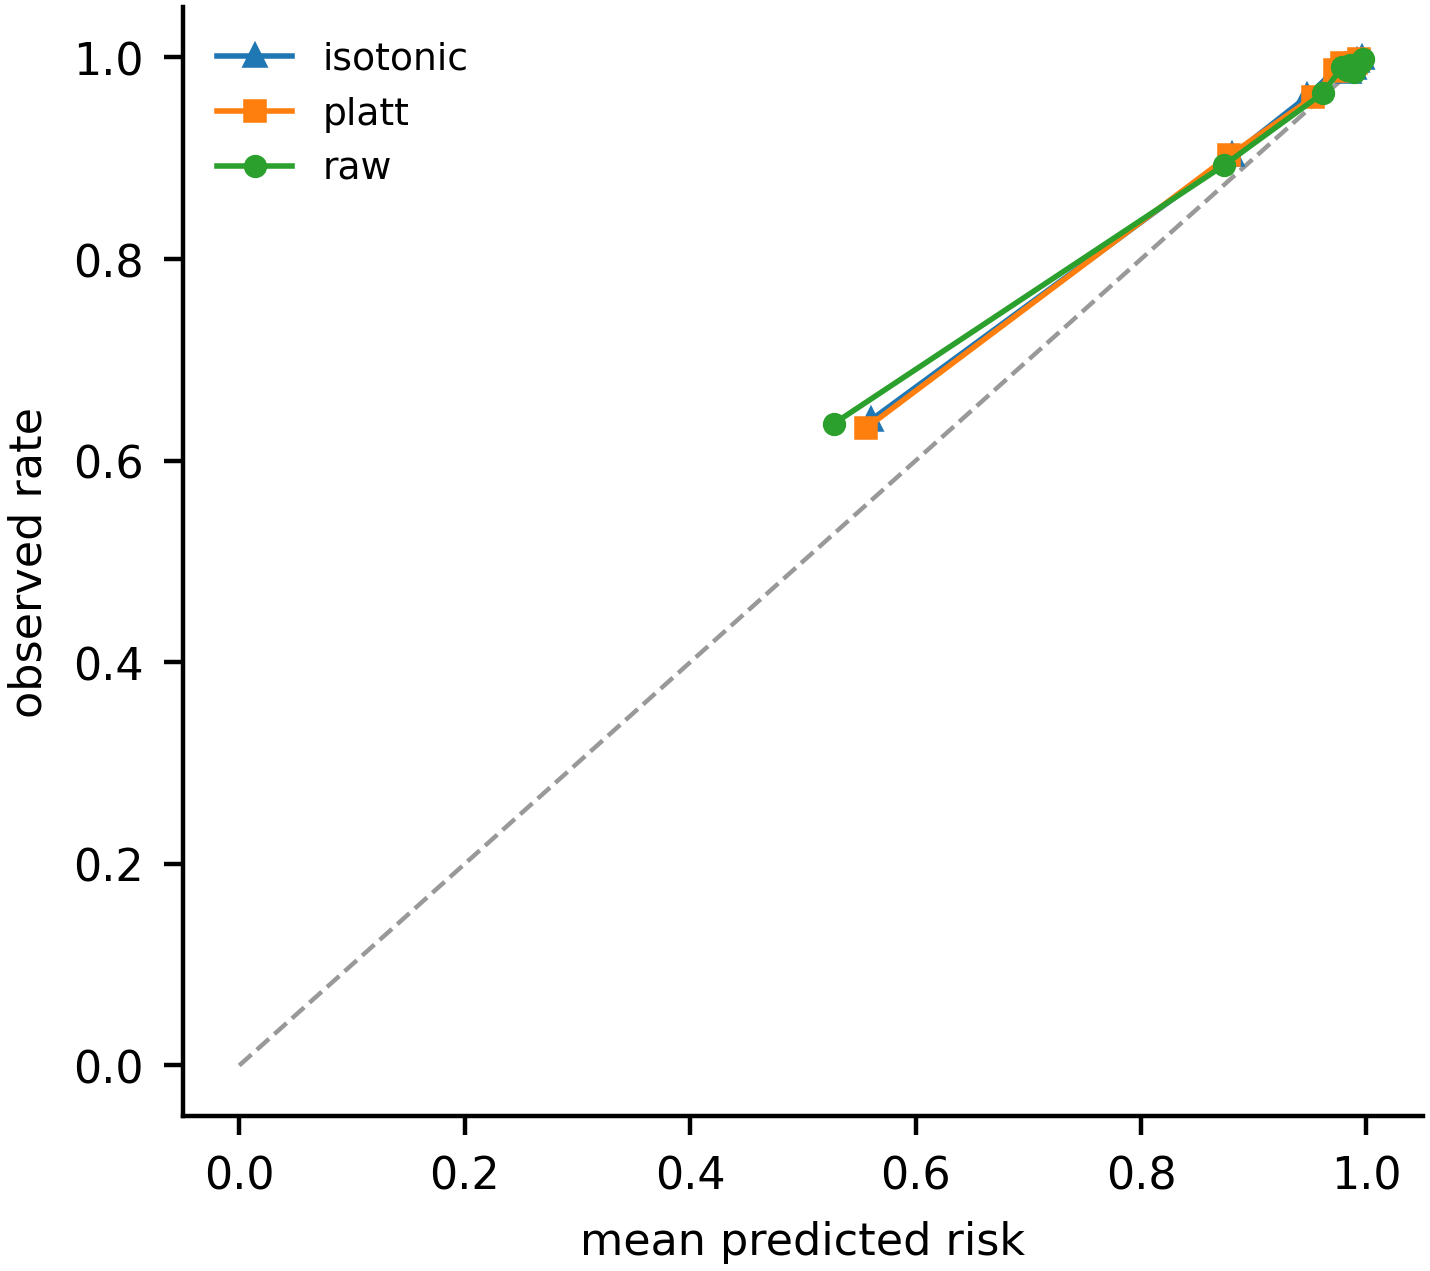
\includegraphics[width=0.72\linewidth]{figS7_calibration.png}
\caption{Calibration at the reference cell on the case study's log, by decile
of predicted risk. The two proper scoring rules on the metric axis --- Brier
skill and the log-loss skill --- read this picture; the two rank-based ones
cannot see it at all (Proposition~\ref{prop:rank}). A pipeline whose
discrimination is adequate and whose calibration is not therefore moves the
increment on some instruments and not others, which is one concrete mechanism
behind the metric axis's contribution to Table~\ref{tab:sobol}.}
\label{fig:calibration}
\end{figure}

The frequency-encoded pipeline is the one that is visibly miscalibrated, with
a slope well below one, and it is also the one whose increment differs most
from the others on the two proper scoring rules. That is the interaction
between the pipeline axis and the metric axis, drawn.

Rolling-origin results are in \texttt{results/s01\_surface.csv} under
\texttt{split = rolling$k$} and enter the decomposition as the split axis;
Supplement~\ref{app:rolling} prints them per fold. The single holdout is not
the best estimate of the increment, and reporting it alone would be a
limitation.
